\chapter{Event Selection \& Background Estimation} \label{chap-EventSelection}

When we finally arrive at a point when we have identified and reconstructed all the objects in the data, as described in Section \ref{chap-EventReconstruction&Simulation}, we impose a set of kinematic and topological cuts to each of the objects in order to provide a subset of the data containing mainly our signal events. The signal sample still contains background events and is corrected in several ways. Simulated MC samples are produced and used to optimise the number of signal events within this sample, and thus rejecting as much background as possible. The selection process, including kinematic, topological, and fiducial cuts on our final state objects is described in detail in the first part of this chapter.

Even though we model data using simulated MC samples, which are an essential tool for modelling distributions in particle physics, this is not always enough to provide a robust and accurate measurement of a process. In this case, additional methods for the calculation of background processes are used to purify our signal sample by removing events that are not in fact our final state signal event. These methods can be MC-driven and data-driven, and both are described in the second part of the chapter in greater detail pertaining to the $t\bar{t}+\gamma$ analysis.  

\section{Event Selection} \label{sec-EventSelection}

Skim
Preselection then photon selection

For the $t\bar{t}+\gamma$ analysis the selection of objects is computed in three stages; A \textbf{skim} is implemented when processing signal and background MC samples in order to reduce the rate of events at analysis level and become much more manageable, a \textbf{pre-selection} of $t\bar{t}$ events is then computed for each final state respectively following the recommended top event selection group reference, and finally the full \textbf{selection} which includes an isolated photon radiated from top quark or its decay products.   

It is important to reconstruct the number of $t\bar{t}$ events before we can include our radiated photon such that our sample is much cleaner. 
The pre-selection events have been constructed by following the CMS recommendation for cut-based selection of top-quark pair events with the requirement of at least two jets of which at least one is a b-tagged jet. Individual objects are reconstructed based on specific criteria, such as electrons, loose electrons, muons, loose muons, jets, and photons. Then an additional set of selection requirements is applied based on the relative positions of the objects ($\Delta R$ cuts). After that, the final decision is made if the event is to be considered in the further analysis. Pre-selection cuts are described in Section \ref{sec-preselection}.

\section{Pre-selection: Selection of $t\bar{t}$ Events} \label{sec-preselection}

The pre-selection steps define our $t\bar{t}$ events before the addition of a radiated photon. The selection follows the recommended selection from the TOP Reference Selections and Recommendations (Run1) \cite{TopEventSelection} designed to select di-lepton final states with two isolated oppositely charged leptons, at least 2 jets where at least one is a b-tagged jet, and two neutrinos from missing transverse energy. All objects in the selection are reconstructed using the PF algorithm as described in Section \ref{subsec-PFAlgorithm}.  


\section{Trigger and Event Cleaning} \label{sec-TriggerAndEventCleaning}

\subsection{Trigger selection}

As the $t\bar{t}+\gamma$ analysis is studied as a di-lepton final state, the requirement of at least two oppositely charged leptons (electrons or muons only) is essential. These datasets are identified by the trigger system (as described in Section \ref{sec-Trigger}) to contain two leptons. Triggers are generally divided into two categories; single object triggers fire on one or more objects of the same flavour passing certain pre-selection requirements, such as p$_T$ and $\eta$, and cross-triggers which select two objects of different flavours as predetermined by the user. For this analysis, both types of triggers are implemented in order to select the three final states in question. The list of trigger paths can be seen in Table \ref{tab-HLTriggers}. 

\begin{table} \label{tab-HLTriggers}
\begin{center}
\begin{tabular}{|c|p{11.5cm}|}
\hline
	\textbf{Final State} & \textbf{High Level Trigger Path} \\
\hline
	$\mu^+\mu^-$ & HLT\_Mu17\_Mu8\_v* \\
	$e^+e^-$ & HLT\_Ele17\_CaloIdT\_CaloIsoVL\_TrkIdVL\_TrkIsoVL
				\_Ele8\_CaloIdT\_CaloIsoVL\_TrkIdVL\_TrkIsoVL\_v* \\
	$e\mu$ & HLT\_Mu17\_Ele8\_CaloIdT\_CaloIsoVL\_TrkIdVL\_TrkIsoVL\_v*, HLT\_Mu8\_Ele17\_CaloIdT\_CaloIsoVL\_TrkIdVL\_TrkIsoVL\_v*s \\
\hline	
\end{tabular}
\caption{Triggers for each di-lepton channel.}
\end{center}
\end{table}

Each trigger path name explains the selection requirements on the objects that it triggers on. The term Mu refers to a reconstructed muon and Ele refers to a reconstructed electron, where the succeeding number represents an associated energy threshold of the particle. For example, the the di-muon channel uses a single flavour object trigger to select two muons and is used with the requirements that one of the muons has a p$_T$ greater than 8 $\GeV$ and the second greater than 17 $\GeV$. The version of the trigger is denoted in the trigger path as v*, as the trigger path changes with the trigger table used. It should be noted that a different trigger version does not in fact require a change in trigger path. At this level the number of energy deposits within the calorimetry is still too large for the trigger rate to be usable, and thus extra selection requirements on the trigger system must be imposed.

A way to reduce the trigger rate is to impose cuts on the energy threshold of the particles in question greater than that required by the trigger, however this holds drawbacks for analyses who then wish to implement tighter cuts within offline analysis. Another method, and one that is used primarily in electron trigger studies, is to reduce trigger rates to a more feasible level is to introduce isolation and Id cuts, the `Iso' and `Id' terms that can be seen in the di-electron and $e\mu$ trigger path names. The objects must then also pass simple isolation and id criteria and thus reducing the trigger rate. The information for each is obtained from both the calorimeter (e.g CaloIso) and tracker (e.g TrkId) by placing requirements on such parameters as the shape of the energy cluster, the total number of energy depositions, and the angular separation between the ECAL and tracker energy deposits. Three categories of selection are implemented for each kinematic cut, and are listed as Tight (T), Loose (L), and Very Loose (VL) as can be seen in the trigger paths. These signify the harshness of the cuts when applied. This can be visualised, for example, in the the di-electron channel where the HLT calls for two electrons, where one must pass an energy threshold of 8 $\GeV$ with a tight requirement on calorimeter Id, and very loose requirements on calorimeter isolation and tracker Id and isolation. The other electron must pass an energy threshold of 17 $\GeV$ with the same calorimeter and tracker isolation and Id cuts.

HLTs are used for the $t\bar{t}+\gamma$ analysis such that if the event does not pass the requirement of the trigger, then it is not included in the calculation. Single object triggers are used for both the di-muon and di-electron channels, and two cross-triggers were used for the $e\mu$ channel as the final state selection requires two oppositely charged leptons (electrons or muons) where one is an electron and the other a muon. The triggers were processed specifically for the $\sqrt{s}=8 \TeV$ data-taking period with 19.6 $\fbinv$.

\subsection{Filtering}

Known anomalies derived from detector and accelerator effects are a prominent feature in the processing of data. To counter these effects we incorporate several `cleaning' filters after trigger selection, but before any further selection cuts are applied. The first of which vetoes on \textbf{beam scraping} and includes a \textbf{tight CSC Beam Halo Filter}. We find that, even with the accuracy and precision that the LHC provides on accelerating bunches of protons, protons have a tendency to diverge radially from the bunch and form what is known as the beam halo that circulates the accelerator with the bunch. In early analyses it was found that the beam halo particles can be picked up in the detectors and be reconstructed as being part of an event in which it is not. Due to sensitivity to beam halo particles in the muon detectors, a filter is introduced based on muon tracking kinematics and thus veto on such events. Beam halo particles can also be removed from the beam within the LHC by introducing collimating blocks around the beam line at various points on the accelerator. This, however, presents another problem in the form of showering as the particles interact with the collimator blocks, beam scraping, and be detected by the experiments. These events are accounted for and removed from analyses by introducing the requirement that at least 25\% of reconstructed tracks within the inner detector pass the high purity threshold (see Section \ref{subsec-ChargedParticleTracking}). 

Similarly, we employ a \textbf{HCAL noise filter} in order remove events with anomalous noise within the HCAL. CMS expects a certain degree of noise, stemming from the electronic of the detector, to be present when recording data, however the majority of anomalous noise is found to originate in the Hybrid Photo-Triodes (HPT) and their corresponding read-out boxes. At the current energy scale this is not a problem as the noise appears as large, isolated energy deposits. Anomalous events have easily-identifiable signatures such as the isolation and isolation of the HCAL readout, and the multiplicity in the read-out boxes. So, if a signal demonstrates very little change in the pulse shape over time, and the read-out boxes display a high multiplicity, then an event is rejected. The next filter system comes in the form of the \textbf{HCAL laser filter}. The need for the laser filter first manifested during the 2011 data taking period when a much greater number of events were observed than was expected - $\sim5000$ htis per event. The HCAL laser filter was then designed and introduced for the 2012 data taking period.  

%%%%%%%%%%%%%%%%%%More

\section{Di-lepton Selection and Vetoes}

For the $t\bar{t}+\gamma$ analysis leptons mark our signature for our final state events. The leptons are taken from the list of PF-reconstructed objects and then required to pass additional selection cuts to refine the events further after trigger selection in Section \ref{sec-TriggerAndEventCleaning}. Along with our signal leptons, a set of `looser' PF objects are selected as veto objects, such that our signal leptons are a subset of these objects. If an event has multiple loose selection leptons then the event is removed from the list of possible signal candidates.

The number of selected leptons differs for each decay mode, and thus three separate selections must be created for the di-muon, di-electron, and mixed channels, respectively. Cuts on leptons vary depending on the channel, but are taken from the recommended values produced by the central `Top Event Selection' group \cite{TopEventSelection}. 

\subsection{Electrons}

PF electron candidates are selected for di-electron and $e\mu$ final states if they have been identified by the GSF method, as described in Section \ref{subsec-ElectronIdentification} and pass the HLT for each channel respectively. The rates are then reduced by imposing a further set of cuts taken from the recommended top reference selection cuts \cite{TOPEGM1}. The cuts are as follows:

\begin{itemize}
	\item Passes a p$_T$ threshold of > 20 \GeV.
	\item Lies within the pseudorapidity region $|\eta| < 2.5$, excluding the EB-EE transition region $1.4442 < |\eta| < 1.5660$.
	\item The transverse IP of the electron (GSF) track with respect to the first offline primary vertex must be less than 0.04 cm. 
	\item Combined relative Particle Flow (PF) $\rho$ corrected isolation in cone 0.3 less than 0.15.
	\item Trigger version of electron multivariate discriminator Trigger MVAID greater than 0.5.
	\item Conversion rejection: there should be no extra tracks pointing in the same direction.
	\item The ratio of energy deposited in the HCAL over the energy deposited in the ECAL to be less than 0.05.
\end{itemize} 

For electrons, an additional identification process is included, which uses a multivariate analysis to combine the information of several variables to produce a discrimination value between -1 and 1, such that the greater the number the more likely the event is to be an electron, (as described in Section \ref{subsec-ElectronIdentification}). Depending on whether the HLT requires an electron or not, a different version of the discriminant is used. 

One of the main criteria for lepton selection is the requirement of isolation. Generally, we define the isolation to be the sum of the p$_T$ of the reconstructed objects within a cone by which we define the radius, and then diving by the p$_T$ of the object. If we find that this produced a small number, then we say that the object is isolated. We must, however, include the effect of event PU into the calculation of isolation, and thus we introduce a correction factor. We are able to remove charged hadron tracks from the isolation sum if they do not originate from the event's primary vertex. For the case of neutral hadrons and photons which originate from PU, an effective area is defined for the electron and then an average energy is subtracted over this area. The effective area is extended into the ECAL due to the emittance of Bremsstrahlung radiation. For the case of electrons, we can define the isolation as so

\begin{equation} \label{eq-RelativeIsolation}
I_{\rho} = \frac{I_{ChargedHadron}+max\left(I_{NeutralHadron} + I_{\gamma} - \rho \cdot Eff.Area_{electron}, 0 \right)}{p_T}
\end{equation}

such that $I_{ChargedHadron}$, $I_{NeutralHadron}$, and $I_{\gamma}$ are the are the isolation cones with a fixed radius of $\Delta R = 0.3$ containing the energy deposits for each category of particle; charged hadron, neutral hadron, and photon isolation. The $\rho$ and $Eff.Area_{electron}$ parameters are the energy density of the event and the effective area for the electron which is calculated by taking the $\eta_{SC}$ and electron p$_T$. 

When a photon produced in collisions interacts with the detector material of the inner tracker it can pair-produce two electrons, thus mimicking the signature of an electron. The false signature has been calculated to represent a large source of fake electrons. The CMS EGamma working group have developed two methods in order to mitigate the fake electron signatures from the hard scattering process: measuring missing hits within the tracker system and measuring associated secondary tracks. The first technique measures the number of hits in the layers of the tracker and looks for any missing hits in the electrons associated track. If there are any missing hits, then the electron is considered as converted and discarded. The second method requires a secondary electron/positron track such that it reconstructs the pair under a certain criteria. If a second track is not found to be within 0.02 cm in the $r - \phi$ plane and the $\cot\theta$ differs by less than 0.02 then the electron is considered a conversion. 

We define a set of loose electron candidates by applying the recommended cuts as for our signal electrons but with less stringent requirements, such that our signal electrons are a subset of the loose electrons. The difference between loose and signal electrons is given by a p$_T$ cut of $> 10 \GeV$, non-triggering ID greater than zero, and several other cuts which are implemented for the identification of signal electrons are not included for loose. The \textbf{loose electrons} are defined to have the following cuts:

\begin{itemize}
	\item Transverse momentum $p_T$ greater than 10 GeV
	\item Absolute value of pseudorapidity less than 2.5
	\item Combined relative Particle Flow (PF) $\rho$ corrected isolation in cone 0.3 less than 0.15
	\item Trigger version of electron multivariate discriminator Non-Trigger MVAID greater than 0
\end{itemize}

\subsection{Muons}

For our \textbf{signal muons}, once they have passed PF selection as described in Section \ref{subsec-MuonReconstruction}, additional cuts taken from the recommended muon physics object group (POG) \cite{TOPMUO1} are imposed as follows:

\begin{itemize}
	\item Transverse momentum p$_T$ greater than 20 \GeV.
	\item Lies within the pseudorapidity region $|\eta| < 2.4$, excluding the EB-EE transition region $1.4442 < |\eta| < 1.5660$.
	\item Combined relative Particle Flow (PF) $\rho$ corrected isolation in cone 0.4 less than 0.2
	% \item At least 5 hits in the tracker (with at least one coming from the pixel detector)
	% \item At least one hit in the muon detector
	\item Identified as a particle flow muon
	\item Identified as both a tracker and global muon
\end{itemize}

The analogous relative isolation for the signal muon candidates is pileup correction and much less complicated to compute. The technique is known as $\Delta \beta$ correction and removes the neutral hadron and photon isolation from the isolation sum within a fixed cone of radius $\Delta R = 0.4$. The relative isolation can be computed as so 

\begin{equation}
I_{\Delta \beta} = \frac{I_{ChargedHadron} + max\left(I_{NeutralHadron} + I_{\gamma} - 0.5 \cdot I_{Pileup}, 0 \right)}{p_T}
\end{equation}

where the $I_{Pileup}$ parameter is the neutral hadron energy within the cone, and the factor of 0.5 is a rough estimation of the ratio of neutral hadron to charged hadron in pileup events. We categorise a muon as being isolated if the isolation sum is less than $I_{\Delta \beta} < 0.2$ within an isolation cone of $\Delta R = 0.4$. 

The production of muons from inn-flight decays is found to be much more prominent in data than is modelled in simulation. This results in a number of fake muons being recorded. In order to account for the number of fakes, the implementation of further cuts is required such that at least one hit is required in each of the pixel detector and muon detectors, and at least 6 hits recorded in the inner tracking system with two corresponding hits in the outer muon system.  

\textbf{Loose Muons} are selected from PF muons failing the muon selection that have, and are selected to have less severe requirements as listed below:

\begin{itemize}
	\item Transverse momentum $p_T$ greater than 10 GeV
	\item Absolute value of pseudorapidity less than 2.5
	\item Combined relative Particle Flow (PF) $\rho$ corrected isolation in cone 0.4 less than 0.2
	% \item At least 5 hits in the tracker (with at least one coming from the pixel detector)
	% \item At least one hit in the muon detector
	\item Identified as a particle flow muon
	\item Identified as both a tracker and global muon
\end{itemize}

\subsection{Corrections to simulated events} \label{subsec-SimulatedEventsCorrection}

\section{Jet Selection and b-tag Requirements} \label{sec-JetSelection}

Jets are reconstructed with the PF AK5 algorithm, anti-$k_T$ with jet size parameter (R) of 5 in the jet reconstruction model, and the following selections are made (PF loose Jet ID). Before applying any selection the following corrections are made to account for imperfect jet energy measurement: Jet Energy Scale correction, and Jet Energy Resolution smearing, as described in Section \ref{subsec-JetReconstruction}. After jets are identified and reconstructed, the following set of cuts are implemented with the requirements:

\begin{itemize}
	\item Transverse momentum greater than 30 GeV
	\item Absolute value of pseudorapidity less than 2.4
	\item Number of constituents greater than 1
	\item Charge multiplicity greater than 0
	\item Neutral hadron fraction of energy less than 0.99
	\item Neutral electromagnetic energy fraction less than 0.99
	\item Charged EM energy fraction less than 0.99
	\item Charged hadron energy fraction greater than 0
\end{itemize}

These cuts help to avoid picking detector noise and ECAL spikes as jets. We also impose a selection criterion that if a lepton lies within a cone of $\Delta R = 0.3$, then the lepton is included within the jet calculation. CMS improves the quality of reconstructed jets by the requirement that the energy deposits from a jet are recorded in both the ECAL and HCAL, where jets that manifest from anomalous deposits of energy in just one of the sub-detector are able to be removed from the sample \cite{CMS-PAS-JME-10-003}.

 \textbf{B-tagged jets} are identified with the Combined Secondary Vertex b-tagging algorithm using the loose working point (CSVL). Event re-weighting is applied to correct for the difference in b-tagging efficiency in data and simulation as explained in Section \ref{subsec-SimulatedEventsCorrection}. The loose working point refers to a b-tagging efficiency of  and a misidentification probability of 24.4\%.

 In each channel the requirement of at least 2 good jets, where a good jet passes all the aforementioned selection requirements, and at least one b-jet. By applying these requirements the contribution from the most prominent backgrounds, $t\bar{t}$ and events with additional loose jets, are removed. 
 

\section{Selection of $t\bar{t}+\gamma$ events} \label{sec-postselection}

From the set of $t\bar{t}$ preselected events in Section \ref{sec-Preselection}, we select only events with a photon candidate present. Main fiducial requirements are implemented as cuts in $\abs{\eta}$ and $E_T$. CMS recommended cuts are added for fiducialisation and photon selection (tight cut-based photon ID 2012 with particle flow based isolation, \cite{CutBasedIsolation2012}).In order to suppress FSR from final state particles a $\Delta R$ cut of photons between jets and leptons is applied. All simulated data is scaled to the luminosity of the recorded data used.  

\begin{description}

\item[Transverse energy] A transverse energy cut of $E_T > 25$ is implemented in order to suppress the numerous low energy fake photons and photons from other vertices other than the primary
vertex. The transverse energy distribution for each channel can be seen on the left in Figs.\ref{fig-nminusoneMuMu} --- \ref{fig-nminusoneEMu}.

\item[Pseudorapidity] An acceptance cut on the fiducial region of just the CMS ECAL barrel (EB), $\abs{\eta} < 1.4442$, is applied to verify that the electromagnetic shower of
the photon will be fully reconstructed. We will not be including the ECAL Endcap (EE) in this analysis due to the difficulty in identifying a photon thus giving very low
statistics.

\end{description}

\subsection{Cut based photon ID}

\begin{description}

\item[Electron Conversion Veto] A boolean to help distinguish an electron from a photon. We should not see a track seed in the pixel detector when identifying a photon. 

\item[Tower Based H/E] The ratio of energy deposited in the Hadronic Calorimeter (HCal) over the fraction of energy deposited in the Electromagnetic Calorimeter(ECal). This cut is
set so that the energy ratio should be less than 5\% (see Fig.\ref{fig-cutbasedMuMu1} right).

\item[Shower Width \sigma_{i\eta i\eta}] The shower shape weighted by energy (see Fig.\ref{fig-cutbasedMuMu1} right), defined as: 

\begin{equation}
\sigma_{i\eta i\eta} = \left(\frac{\sum(\eta_i - \bar{\eta})\omega_i}{\sum\omega_i}\right)^{1/2};  \bar{\eta} = \frac{\sum\eta_i\omega}{\sum\omega_i};  \omega_i = \text{max}\left(0, 4.7 +
\text{log}\frac{E_i}{E_{5x5}}\right).
\end{equation}

\item[Charged Hadron Isolation] The isolation of charged hadrons with energy density correction, $\rho$, applied. Cut given as $I_{char.had} < 1.5 GeV + 0.04*E_T(\gamma)$. See Fig.\ref{fig-cutbasedMuMu1}.

\item[Neutral Hadron Isolation] The isolation of neutral hadrons with energy density correction , $\rho$, applied. Cut given as $I_{neut.had} < 1.0 GeV + 0.005*E_T(\gamma)$. See Fig.\ref{}.

\item[Photon Isolation] The isolation of the photon $I_{\gamma}$, with energy density correction applied. Cut given as $I_{\gamma} < 1.0 GeV + 0.005*E_T(\gamma)$. See
Fig.\ref{}.

\item[super-cluster Footprint-removed Charged Hadron Isolation] The super-cluster footprint-removed isolation of charged hadrons with energy density correction, $\rho$, applied.
Cut given as $I_{char.had}(SCFR) < 5 \ \text{GeV} $. See Fig.\ref{fig-cutbasedMuMu1}.

\item[super-cluster Footprint-removed Neutral Hadron Isolation] The super-cluster footprint-removed isolation of neutral hadrons with energy density correction , $\rho$, applied.
Cut given as $I_{neut.had} < 1.0 GeV + 0.005*E_T(\gamma)$. See Fig.\ref{}.

\item[super-cluster Footprint-removed Photon Isolation] The super-cluster footprint-removed isolation of the photon $I_{\gamma}$, with energy density correction applied. Cut given
as $I_{\gamma} < 1.0 GeV + 0.005*E_T(\gamma)$. See Fig.\ref{}.

\end{description}

\subsubsection{FSR suppression}

\begin{description}
\item[\Delta R(\gamma, leptons)] In order to diminish FSR in final state leptons, e.g photons radiated off high $p_T$ muons, a minimum distance criterion in the $\eta - \phi$ plane is implemented. The cut is given as $\Delta R(\gamma, leptons) > 0.3$.

\item[\Delta R(\gamma, jets)] In order to reduce FSR in final state partons a minimum distance criterion in the $\eta - \phi$ plane is implemented. The cut is given as $\Delta R(\gamma, jets) > 0.3$.

\item[\Delta R(leptons, jets)] In order to reduce FSR in final state partons a minimum distance criterion in the $\eta - \phi$ plane is implemented. The cut is given as $\Delta R(leptons, jets) > 0.3$.
\end{description}

A significance test was performed in an attempt to optimise the $\Delta R$ cut between final state leptons and jets, however this proved inconclusive due to an initial cut of $\Delta R > 0.1$ at generator level.

\subsection{Super-cluster footprint-removal for photon isolation}

\begin{figure} \label{fig-SCFR}
\begin{center}
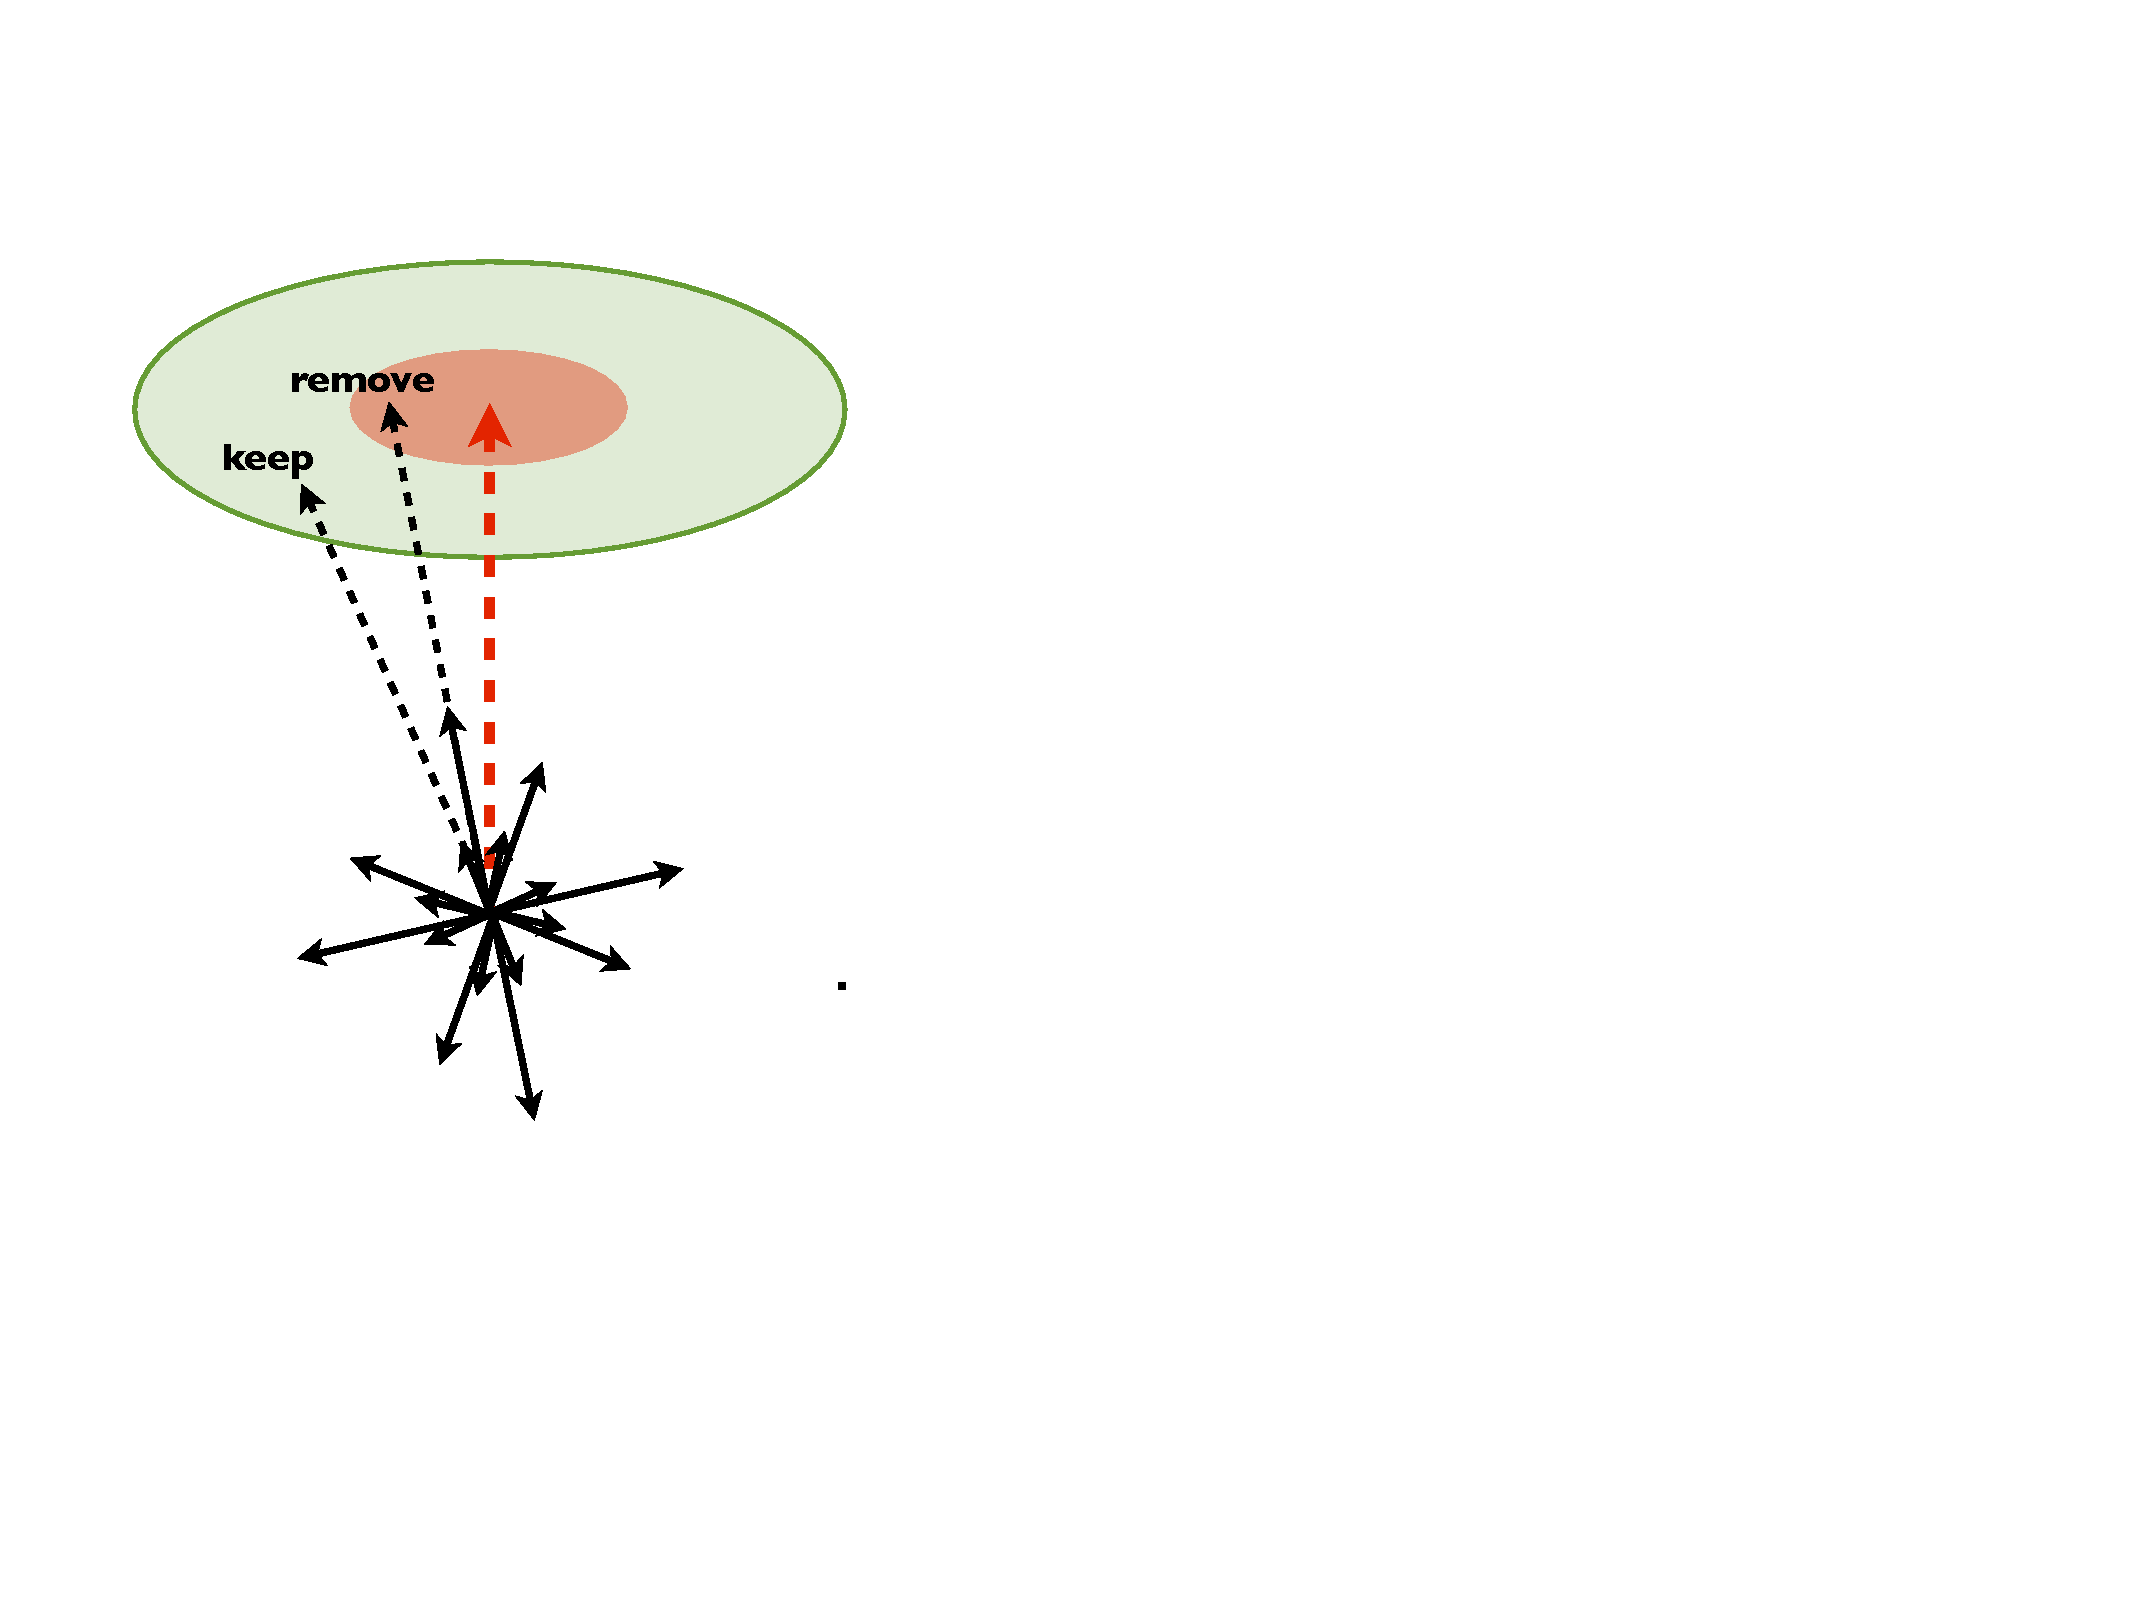
\includegraphics[width=0.4\textwidth]{Figures/RandomCone3.pdf}
\caption{}
\end{center}
\end{figure}

\section{Background Estimation}

\begin{figure} \label{fig-RandomConeIsolation}
\begin{center}
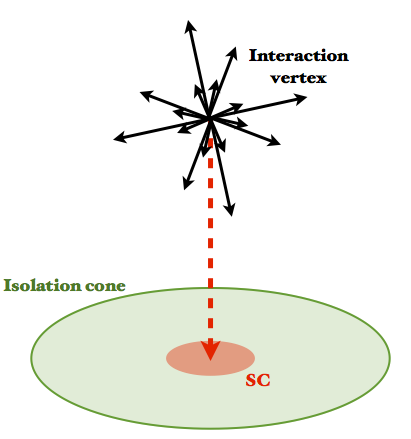
\includegraphics[width=0.45\textwidth]{Figures/RandomCone1.png}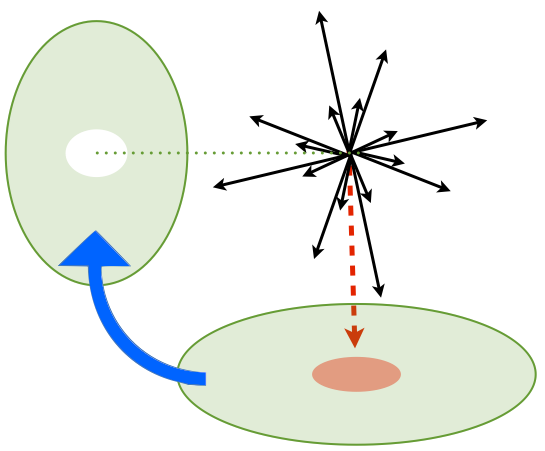
\includegraphics[width=0.55\textwidth]{Figures/RandomCone2.png}
\caption{}
\end{center}
\end{figure}

\begin{sidewaystable} \label{tab-datasets}
\begin{center}
\begin{tabular}{|l|c|c|}
\hline
	\textbf{Dataset} & \textbf{Run Range} & \textbf{Integrated Luminosity ($pb^{-1}$)}\\
\hline
	/DoubleMuParked/Run2012A-22Jan2013-v1/AOD &  & 876 \\
	/DoubleMuParked/Run2012B-22Jan2013-v1/AOD &  & 4412 \\
	/DoubleMuParked/Run2012C-22Jan2013-v1/AOD &  & 7017 \\
	/DoubleMuParked/Run2012D-22Jan2013-v1/AOD &  & 7369 \\
\hline
	Total & & 19.7\\	
\hline
	/DoubleElectron/Run2012A-22Jan2013-v1/AOD &  & 875 \\
	/DoubleElectron/Run2012B-22Jan2013-v1/AOD &  & 4412 \\
	/DoubleElectron/Run2012C-22Jan2013-v1/AOD &  & 7055 \\
	/DoubleElectron/Run2012D-22Jan2013-v1/AOD &  & 7369 \\
\hline
	Total & & 19.7\\	
\hline
	/MuEG/Run2012A-22Jan2013-v1/AOD &  & 876 \\
	/MuEG/Run2012B-22Jan2013-v1/AOD &  & 4411 \\
	/MuEG/Run2012C-22Jan2013-v1/AOD &  & 7055 \\
	/MuEG/Run2012D-22Jan2013-v1/AOD &  & 7360 \\
\hline
	Total & & 19.7\\	
\hline	
\end{tabular}	
\caption{Dataset information for each run in each respective decay channel.}
\end{center}
\end{sidewaystable}

